\documentclass[11pt]{beamer}
\usetheme{OIE}
\usepackage[utf8]{inputenc}
\usepackage[german]{babel}
\usepackage[T1]{fontenc}
\usepackage{amsmath}
\usepackage{amsfonts}
\usepackage{amssymb}
\usepackage{tikz}
\usepackage{graphicx}
\usepackage{color}
\usepackage{booktabs}
\usepackage{pifont}
\usepackage{xcolor}
\usepackage{fancyvrb}
\usepackage[natbib=true,backend=bibtex,style=authoryear]{biblatex}
\author{Dominik Both, Tonio Weidler}
\title{Open Information Extraction}
%\setbeamercovered{transparent} 
%\setbeamertemplate{navigation symbols}{} 
%\logo{} 
\institute{Institut für Computerlinguistik, Universität Heidelberg} 
\date{15.07.2016} 
\subject{} 
\definecolor{lightgray}{gray}{0.8}

\begin{document}

% AUTOMATISMEN
\AtBeginSection{\frame{\sectionpage}}
\AtBeginSubsection{\frame{\subsectionpage}}


% TEMPLATING
\setbeamertemplate{title page}{
	\center 
		\begin{beamercolorbox}[center]{part title}
	      \Huge\inserttitle\par
	    \end{beamercolorbox}
	    \vspace{15pt}
		\insertauthor\\
		\vspace{15pt}		
		Proseminar \textit{Text Mining}\\
		Andrea Zielinski\\
		\vspace{15pt}
		\insertinstitute, \insertdate
}

\defbeamertemplate{section page}{wiqe}[1][]{%
  \begin{centering}
    \begin{beamercolorbox}[center]{part title}
      \Huge\insertsection\par
    \end{beamercolorbox}
  \end{centering}
}

\defbeamertemplate{subsection page}{wiqe}[1][]{%
  \begin{centering}
    \begin{beamercolorbox}[center]{}
      \usebeamerfont{subsection title}\usebeamercolor[fg]{subsection name}\insertsection\par
    \end{beamercolorbox}
    \begin{beamercolorbox}[sep=2pt,center]{part title}
		\huge\insertsubsection\par
    \end{beamercolorbox}
  \end{centering}
}
\setcounter{tocdepth}{1}
\setbeamertemplate{section page}[wiqe]
\setbeamertemplate{subsection page}[wiqe]

% COMMANDS
\newcommand{\hitem}{
	\item[\color{lightgray}\rule{0.5em}{0.5em}]
}

\begin{frame}
\titlepage
\end{frame}

\begin{frame}{Strukturierung}
    \tableofcontents
\end{frame}

\section{Introduction}
\section{OIE - Principles}
	\subsection{Motivation}
	\subsection{Methods}
	\subsection{Data Representation}
		\begin{frame}{Standard Patterns}
			\begin{center}
				\includegraphics[scale=0.5]{img/oie-pattern.png}\\
				\vspace{15pt}
				\textbf{Argument A} is in a directed \textbf{relation} to \textbf{Argument B}.
			\end{center}
		\end{frame}
		
		\begin{frame}{Unnormalized Annotation}
			\begin{center}
				(argument\_a, predicate\_x, argument\_b)\\
				(argument\_a, predicate\_y, argument\_c)\\
				(argument\_a, predicate\_y, argument\_d)
			\end{center}
			\vspace{15pt}
			\textbf{Problems}\\
			\begin{itemize}
				\item redundant
				\item unnormalized
				\item can only produce binary predicates
			\end{itemize}
		\end{frame}
		
		\begin{frame}{RDF and Linked Data}
			\begin{block}{Resource Description Framework}
				Models propositions by constructing \textit{triples} including \textbf{Subjects}, \textbf{Objects} and \textbf{Predicates}\\
				Generates a directed graph
			\end{block}
			\vspace{10pt}
			\begin{center}
				:subject :predicate :object.
				\vspace{10pt}
				\includegraphics[scale=0.5]{img/oie-rdf-triple.png}
			\end{center}
		\end{frame}
		
		\begin{frame}{RDF Concepts and Notation}
			\begin{itemize}
				\item \textbf{URIs}\\
					identifies ressources (S, R, O) distinctivly and references further informations (triples)
				\item \textbf{Conclusions}\\
					allows to draw conclusions using rules
				\item \textbf{Turtle}\\
					allows syntax abbreviations
				\item \textbf{Queries}\\
					can be searched by querying (eg SPARQL)
				
			\end{itemize}
		\end{frame}
		
		\begin{frame}{Basic relations (built in)}
			\begin{table}[]
				\centering
				\begin{tabular}{ll}
				\textbf{Relation} & \textbf{Functionality} \\
				rdf:type (a)      & x is of type y         \\
				owl:sameAs        & x equals y           	
				\end{tabular}
			\end{table}
		\end{frame}
		
		\begin{frame}[fragile]{RDF Syntax}
			\begin{verbatim}
				dbr:Barack_Obama a foaf:person, :President;
				    dbo:spouse dbr:Michelle_Obama.
				dbr:Bernie_Sanders dbo:birthPlace dbr:New_York, 
				                                  dbr:Brooklyn;
				dbr:Brooklyn dbo:isPartOf dbr:New_York 	
			\end{verbatim}
		\end{frame}
		
		\begin{frame}{... as Graph}
			\begin{center}
				\includegraphics[scale=0.4]{img/oie-rdf-example.png}
			\end{center}			
		\end{frame}
\section{Example: LODifier}
	\begin{frame}{LODifier: Generating Linked Data from Unstructured Text (Augenstein et al., 2012}
		\begin{center}
			Generate an RDF Graph from unstructured Text\\
			\vspace{15pt}
			\textbf{Past Approaches:} Use Patterns to trade recall for precision\\
			\textbf{LODifier:} Process the entire text
		\end{center}
	\end{frame}
	\subsection{Architecture}
		\begin{frame}{Architecture}
			\begin{center}
				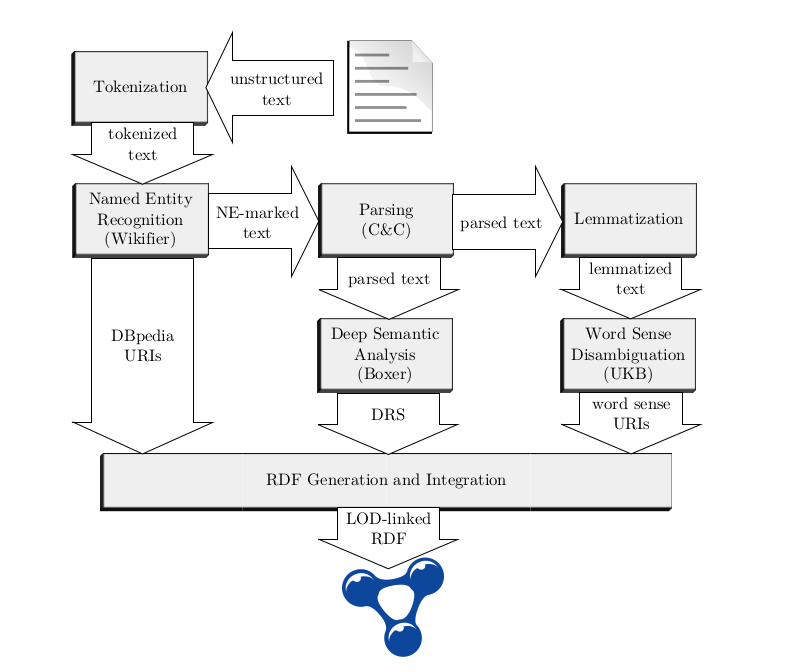
\includegraphics[scale=0.25]{img/oie-lodifier-architecture.png}
			\end{center}
		\end{frame}
		
		\begin{frame}{Approach}
			\begin{enumerate}
				\item \textbf{Parse} the input text (POS, Treetagging, NER)
				\item Apply \textbf{Deep Semantic Analysis} to get relations
				\item Enrich NEs and words with \textbf{URIs} (DBpedia and WordNet)
				\item Forge an \textbf{RDF Graph} of this information
			\end{enumerate}					
		\end{frame}
		
		\begin{frame}{How does it happen?}
			Lets go through the process step-by-step!\\
			\vspace{15pt}
			\textbf{Example Text:}\\
			The New York Times reported that John McCarthy died. He invented the programming language LISP.\\
			\tiny{example taken from Augenstein et al., 2012}			
		\end{frame}
	\subsection{Preprocessing}
		\begin{frame}{Named Entity Recognition - Wikifier}
			\begin{block}{Wikifier}
				Recognizes NE and replaces them with the Wikipedia Page Link\\
				Disambiguates by comparing links between pages.
			\end{block}
			\vspace{15pt}
			\textbf{Example Text Output:}\\
			\textcolor{green}{[The New York Times]} reported that \textcolor{green}{[John McCarthy (computer scientist)|John McCarthy]} died. He invented the \textcolor{gray}{[Programming language|programming language]} \textcolor{gray}{[Lisp (programming language)|LISP]}.
		\end{frame}
		
		\begin{frame}{Parsing Syntax - C\&C}
			\begin{block}{C\&C Parser}
				Syntactical Parser that tags POS and builds Parse Trees (CCG).
			\end{block}
		\end{frame}
		
		\begin{frame}[fragile]{Parsing - Output}
			\begin{Verbatim}[fontsize=\tiny]
				ccg(1, rp(s:dcl,
				    ba(s:dcl,
				      lx(np, n,
				        t(n, ’The_New_York_Times’, ’The_New_York_Times’, ’NNS’, ’I-NP’, ’O’)),
				      fa(s:dcl\np,
				        t((s:dcl\np)/s:em, ’reported’, ’report’, ’VBD’, ’I-VP’, ’O’),
				        fa(s:em,
				          t(s:em/s:dcl, ’that’, ’that’, ’IN’, ’I-SBAR’, ’O’),
				          ba(s:dcl,
				           lx(np, n,
				             t(n, ’John_McCarthy’, ’John_McCarthy’, ’NNP’, ’I-NP’, ’I-PER’)),
				           t(s:dcl\np, ’died’, ’die’, ’VBD’, ’I-VP’, ’O’))))),
				    t(period, ’.’, ’.’, ’.’, ’O’, ’O’))).				
				ccg(2, rp(s:dcl,
				    ba(s:dcl,
				      t(np, ’He’, ’he’, ’PRP’, ’I-NP’, ’O’),
				      fa(s:dcl\np,
				        t((s:dcl\np)/np, ’invented’, ’invent’, ’VBD’, ’I-VP’, ’O’),
				        fa(np:nb,
				          t(np:nb/n, ’the’, ’the’, ’DT’, ’I-NP’, ’O’),
				          fa(n,
				            t(n/n, ’programming_language’, ’programming_language’, ’NN’, ’I-NP’, ’O’),
				            t(n, ’LISP’, ’LISP’, ’NNP’, ’I-NP’, ’O’))))),
				    t(period, ’.’, ’.’, ’.’, ’O’, ’O’))).
			\end{Verbatim}
		\end{frame}
		
		\begin{frame}{Find Relations - Boxer}
			\visible<1-3>{\begin{block}{Boxer}
				Creates DRSs from C\&C Output
			\end{block}}

			\visible<2-3>{\begin{block}{Discours Representation Structure (DRS)}
				Represents the discourse via \textit{relations} between \textit{entities}\\
				Allows referencing over the entire discourse
			\end{block}}
			
			\visible<3>{
				\vspace{5pt}
				\textbf{Boxers DRS Relations (Conditions):}\\
				\begin{itemize}
					\item \textbf{Unary Relations (Classes):} eg. \textit{topic}, \textit{person}, \textit{event}, \textit{male}, ... + all verbs
					\item \textbf{Binary Relations:} agent, patient, ... (semantic roles)
				\end{itemize}							
			}
		\end{frame}	
				
		\begin{frame}{Boxer Output}
			\begin{center}
				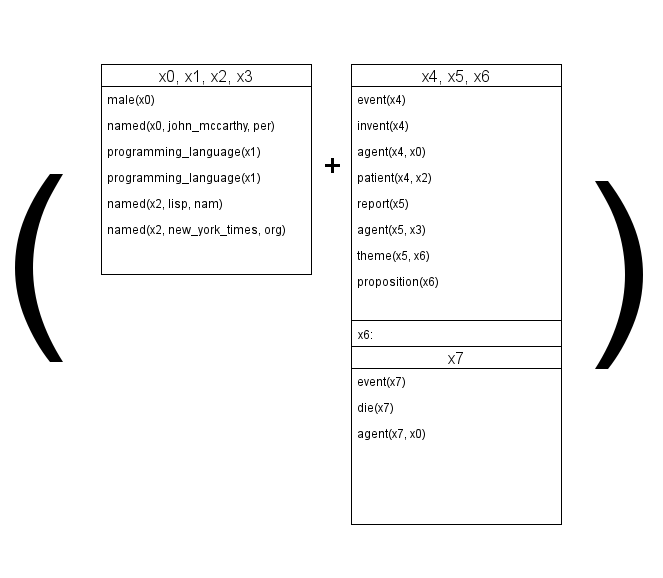
\includegraphics[scale=0.3]{img/oie-boxer-output.png}
			\end{center}
		\end{frame}
		
		\begin{frame}{Assign WordNet URIs}
			\begin{block}{RDF WordNet}
				\textbf{WN:} Lexicography containing senses linked by semantic relations\\
				\textbf{RDF WN:} LD Representation of WN providing URIs for words
			\end{block}
			
			\textbf{Steps:}\\
			\begin{enumerate}
				\item Lemmatization
				\item WSD (UKB)
				\item Assign RDF WN URIs to word senses			
			\end{enumerate}						
		\end{frame}		
		
		\begin{frame}{Preprocessing Result}
			\textbf{We now have ...}
			\begin{itemize}
				\item URIs for all NEs
				\item URIs for all (disambiguated) words
				\item Relations between entities (those URIs)
			\end{itemize}
		\end{frame}				
		
	\subsection{RDF Construction}

		\begin{frame}{What now?}
			\begin{center}
				Let's now construct the RDF Graph from this information!
			\end{center}
		\end{frame}			

		\begin{frame}{Namespaces/Vocabularies}
			LODifier creates several namepaces:
			\begin{itemize}
				\item drsclass:
				\item class:
				\item drsrel:
				\item ne:
				\item reify:
			\end{itemize}
			
			And uses standard namespaces:
			\begin{itemize}
				\item rdf:
				\item owl:
			\end{itemize}
			
			As well as the two ontologies:
			\begin{itemize}
				\item wn30:
				\item dbpedia:
			\end{itemize}
		\end{frame}			

	\subsection{Conclusions}
\section{OIE Systems in Context}
	\subsection{Comparison}
	\subsection{Evaluating the Approaches}
\section{Conclusion}
	\subsection{Problems and Obstacles}
	\subsection{Future Opportunities}

\end{document}